% =====================================================================
% Guía del estudiante -- Trigonometría 10° -- Trimestre I
% María Mercedes Cantillo · Colegio San Alberto Magno
% ---------------------------------------------------------------------
% Plan: guia-periodo-I-medir-lo-inalcanzable.plan.md y la propuesta del
% trimestre I en curriculo/plan-anual.md (sesiones 009-048). Cada \tema
% tiene \label{tema:...} para que las clases lo citen con \refguia{tema:...}.
% No borrar el .aux de esta guía.
%
% Compilar:  latexmk -pdf guia-periodo-I-medir-lo-inalcanzable.tex
% =====================================================================
\documentclass[11pt]{article}
\makeatletter\def\input@path{{../../../../plantillas/estilo/}}\makeatother
\usepackage{mmcantillo}

% ======================== DATOS DE LA GUÍA ============================
\tipodocumento{Guía del estudiante}
\asignatura{Trigonometría}
\titulo{Triángulos, ángulos y arcos}
\grado{10°}
\periodo{I}
\hiloconductor{Medir lo inalcanzable}
% ======================================================================
% Plan del trimestre aprobado por la docente el 2026-09-18. Esta guía es todavía el borrador de
% la generación rápida del 2026-09-14: falta rehacerla con el proceso de tres etapas.
% DBA: matematicas grado 10 · DBA 4 — Comprende y utiliza funciones para modelar
%      fenómenos periódicos y justifica las soluciones. (Evidencia 1 y comienzo de la 3.)

\begin{document}

\encabezado

% ---------------------------------------------------------------------
% 1. Frase introductoria
% ---------------------------------------------------------------------
% verificado: https://it.wikisource.org/wiki/Il_Saggiatore/6 — «Egli è scritto in lingua matematica, e i caratteri son triangoli, cerchi, ed altre figure geometriche, senza i quali mezi è impossibile a intenderne umanamente parola»
\frase{[El universo] está escrito en lengua matemática, y sus caracteres son
triángulos, círculos y otras figuras geométricas, sin los cuales es imposible
entender humanamente una palabra.}
{Galileo Galilei, \emph{El ensayador} (1623), cap.~6, trad. propia~\cite{galileo1623}}

% ---------------------------------------------------------------------
% 2. Introducción
% ---------------------------------------------------------------------
\seccion{Introducción}

¿Cómo se mide la altura de una montaña sin subirla, el ancho de un río sin
mojarse o el tamaño de la Tierra sin darle la vuelta? Con un lado conocido y
unos cuantos ángulos. Esa es la idea de la \textbf{trigonometría}, palabra
griega que significa «medida del triángulo». En este trimestre aprenderemos a
relacionar los lados y los ángulos de un triángulo rectángulo, a resolver
problemas de medición indirecta y a mirar los ángulos de una forma nueva: como
giros, medidos en grados o en radianes, que recorren arcos de un círculo.

Nuestro hilo conductor es \emph{medir lo inalcanzable}: la historia de quienes
midieron lo que no se podía tocar. Empieza con Tales frente a una pirámide,
sigue con Eratóstenes midiendo la Tierra con una sombra, con Hiparco y sus
tablas, con Hipatia revisando cálculos en Alejandría, con una expedición que
pasó nueve años triangulando los Andes cerca de Quito, y termina en nuestro
país, con los mapas de la Comisión Corográfica.

\textbf{Al terminar este trimestre podrás:}
\begin{itemize}
  \item definir seno, coseno y tangente de un ángulo agudo y explicar por qué no
        dependen del tamaño del triángulo;
  \item usar los valores exactos de $30^\circ$, $45^\circ$ y $60^\circ$;
  \item resolver triángulos rectángulos y problemas de medición indirecta;
  \item medir ángulos como giros, en grados y en radianes, y calcular arcos y sectores;
  \item ubicar en el círculo unitario el punto que corresponde a un ángulo.
\end{itemize}

Este trimestre trabaja un Derecho Básico de Aprendizaje del Ministerio de
Educación Nacional~\cite{mendba}, que se completará durante todo el año:

\begin{dba}[Grado 10 · DBA 4]
Comprende y utiliza funciones para modelar fenómenos periódicos y justifica las
soluciones.
\end{dba}

En este trimestre atendemos dos de sus evidencias: \emph{reconoce el
significado de las razones trigonométricas en un triángulo rectángulo para
ángulos agudos, en particular, seno, coseno y tangente}, y el comienzo de
\emph{calcula algunos valores de las razones seno y coseno para ángulos no
agudos, auxiliándose de ángulos de referencia inscritos en el círculo unitario}.

% ---------------------------------------------------------------------
% 3. Marco teórico
% ---------------------------------------------------------------------
\seccion{Marco teórico}

\subsubsection*{Tales y la sombra de la pirámide}

A Tales de Mileto (siglo VI a.\,C.) se le atribuye haber medido la altura de
las pirámides de Egipto por su sombra. La anécdota la cuentan autores que
vivieron siglos después: según Diógenes Laercio, que cita a Jerónimo, y según
Plinio, Tales esperó el momento del día en que la sombra de un cuerpo mide lo
mismo que el cuerpo; según Plutarco, clavó un palo en el extremo de la sombra
de la pirámide y comparó los dos triángulos que forman los rayos del Sol. Esta
segunda versión es la idea de los \textbf{triángulos semejantes}, la base de
todo este trimestre~\cite{mactutortales}.

\subsubsection*{Eratóstenes mide la Tierra}

Eratóstenes de Cirene (276--194 a.\,C.), director de la Biblioteca de
Alejandría, comparó la sombra del mediodía del solsticio de verano en Siena
(hoy Asuán) y en Alejandría. En Alejandría los rayos formaban un ángulo de
$7^\circ\,12'$ con la vertical, $\frac{1}{50}$ de una vuelta; así calculó que la
circunferencia de la Tierra medía $250\,000$ estadios. Su libro se perdió: lo
conocemos por lo que cuentan Cleómedes, Teón de Esmirna y Estrabón. Qué tan
bueno fue su resultado depende de cuánto medía un estadio, algo que todavía se
discute~\cite{mactutoreratostenes}.

\subsubsection*{Hiparco y la primera tabla}

Hiparco (c.~190--120 a.\,C.), que trabajó probablemente en Rodas, construyó una
\textbf{tabla de cuerdas}: para cada ángulo central de un círculo dividido en
$360$ grados, la longitud de la cuerda que lo cierra. Es el primer ejemplo
conocido de una tabla trigonométrica, y algunos historiadores lo consideran el
fundador de la trigonometría~\cite{mactutorhiparco}. Siglos después, Ptolomeo
recogió ese trabajo en el \emph{Almagesto}.

\subsubsection*{Hipatia revisa los cálculos}

Hacia el año 400, en Alejandría, \textbf{Hipatia} enseñaba matemáticas,
astronomía y filosofía. Ayudó a su padre, Teón, a escribir un comentario en
once libros al \emph{Almagesto}~\cite{mactutorhipatia}. El título del libro III
del comentario la nombra:

% verificado: https://www.encyclopedia.com/people/philosophy-and-religion/philosophy-biographies/hypatia — inscripción de Teón, Comentario al Almagesto III: «the edition having been proof-read by the philosopher Hypatia, my daughter»; analizada en Cameron (1990), GRBS 31, 103–127
\begin{cita}{Teón de Alejandría, título del comentario al libro III del \emph{Almagesto}, trad. propia de la versión inglesa; véase~\cite{cameron1990}}
[\ldots] en la edición revisada por la filósofa Hipatia, mi hija.
\end{cita}

Los historiadores discuten cuánto aportó ella a ese trabajo; lo seguro es que
una mujer revisaba, hace dieciséis siglos, los cálculos de la astronomía más
avanzada de su tiempo~\cite{cameron1990}. Murió asesinada en Alejandría en
415~\cite{mactutorhipatia}.

\subsubsection*{La Misión Geodésica: triangular los Andes}

En el siglo XVIII se discutía la forma de la Tierra: según Newton, achatada en
los polos; según los seguidores de Descartes, alargada. Para decidirlo, la
Academia de Ciencias de París envió en 1735 a Louis Godin, Pierre Bouguer y
Charles-Marie de La Condamine a medir un arco de meridiano cerca del ecuador.
El rey de España nombró a dos jóvenes marinos, Jorge Juan y Antonio de Ulloa,
para acompañarlos~\cite{mactutorlacondamine, mactutorjuan}. Entre Quito y
Cuenca midieron una cadena de triángulos: una sola base, de más de 12~km, en la
llanura de Yaruquí, y todo lo demás con ángulos. Trabajaron allí hasta 1744 y
cubrieron unos $3^\circ$ de latitud; sus mediciones apoyaron la idea de Newton
de una Tierra achatada en los polos~\cite{mactutorjuan}.

\subsubsection*{Codazzi y la Comisión Corográfica}

El 1 de enero de 1850, el gobierno de la Nueva Granada firmó un contrato con
Agustín Codazzi, geógrafo militar nacido en Lugo (Italia) en 1793, para
describir el país y levantar sus mapas. Codazzi recorrió provincia por
provincia hasta su muerte, el 7 de febrero de 1859; con sus datos se
publicaron en 1865 la \emph{Carta geográfica} y el \emph{Atlas de los Estados
Unidos de Colombia}~\cite{bnc}.

Las definiciones, los ejemplos y la mayoría de los ejercicios de esta guía
están adaptados de la guía de apoyo de Adriana Quintero Palomino~\cite{quintero}.

% ---------------------------------------------------------------------
% 4. Temas
% ---------------------------------------------------------------------
\tema{Razones trigonométricas}\label{tema:razones}

\begin{hilo}
Egipto, siglo VI a.\,C. Tales clava un palo en la arena. El palo y su sombra
forman un triángulo rectángulo pequeño; la pirámide y la suya, uno enorme. Los
rayos del Sol llegan con la misma inclinación a los dos, así que los triángulos
son semejantes: basta medir el pequeño para conocer el grande.
\end{hilo}

En un triángulo rectángulo, los lados se nombran respecto a un ángulo agudo
$\theta$: la \textbf{hipotenusa} (frente al ángulo recto), el \textbf{cateto
opuesto} (frente a $\theta$) y el \textbf{cateto adyacente} (el otro lado de
$\theta$).

\begin{center}
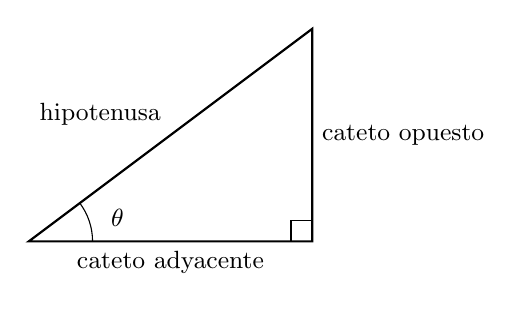
\begin{tikzpicture}[scale=0.9, every node/.style={font=\small}]
  \draw[thick] (0,0) -- (4,0) -- (4,3) -- cycle;
  \draw (3.7,0) -- (3.7,0.3) -- (4,0.3);
  \node[below] at (2,0) {cateto adyacente};
  \node[right] at (4,1.5) {cateto opuesto};
  \node[above left] at (2,1.5) {hipotenusa};
  \draw (0.9,0) arc (0:36.87:0.9);
  \node at (1.25,0.33) {$\theta$};
\end{tikzpicture}
\end{center}

\begin{definicion}[Razones trigonométricas de un ángulo agudo]
\[
  \sen\theta = \frac{\text{cateto opuesto}}{\text{hipotenusa}}, \qquad
  \cos\theta = \frac{\text{cateto adyacente}}{\text{hipotenusa}}, \qquad
  \tg\theta = \frac{\text{cateto opuesto}}{\text{cateto adyacente}}.
\]
\end{definicion}

\textbf{¿Dependen del tamaño del triángulo?} No. Dos triángulos rectángulos con
el mismo ángulo agudo $\theta$ son semejantes: si los lados del grande son $k$
veces los del pequeño, en cada razón se multiplican por $k$ el numerador y el
denominador, y la razón no cambia. Por eso $\sen\theta$, $\cos\theta$ y
$\tg\theta$ dependen \emph{solo del ángulo}.

% Ejercicio: razones-trigonometricas-10-013
\begin{ejemplo}[Hallar un lado con una razón]
En un triángulo rectángulo la hipotenusa mide $35$ y uno de los ángulos agudos
mide $29^\circ$. El cateto $x$ opuesto a ese ángulo cumple
$\sen 29^\circ = \frac{x}{35}$, así que $x = 35\sen 29^\circ \approx \num{17,0}$.
\end{ejemplo}

\begin{aplicacion}[La calculadora científica]
La calculadora trae guardadas las razones de cualquier ángulo: en modo grados
(DEG), la tecla \texttt{sin} de $30$ da $0{,}5$. Las teclas
$\texttt{sin}^{-1}$, $\texttt{cos}^{-1}$ y $\texttt{tan}^{-1}$ hacen lo contrario:
dan el ángulo agudo que tiene esa razón. Si una respuesta sale rara, revisa
primero que la calculadora esté en DEG y no en RAD.
\end{aplicacion}

\begin{preguntas}
% Ejercicio: razones-trigonometricas-10-001, razones-trigonometricas-10-003, razones-trigonometricas-10-005
\pregunta Usa la calculadora (en modo grados) para evaluar, con cuatro decimales:
\begin{opciones*}(3)
  \item $\sen \num{41,3}^\circ$
  \item $\tg \num{54,4}^\circ$
  \item $\cos \num{49,2}^\circ$
\end{opciones*}
\espacio{1.5cm}
% Ejercicio: razones-trigonometricas-10-007, razones-trigonometricas-10-009
\pregunta Con la calculadora, encuentra el ángulo agudo $\theta$ (en grados, a la
décima) tal que:
\begin{opciones*}(2)
  \item $\sen\theta = \num{0,2164}$
  \item $\tg\theta = \num{0,3096}$
\end{opciones*}
\espacio{1.5cm}
% Ejercicio: razones-trigonometricas-10-014
\pregunta En un triángulo rectángulo la hipotenusa mide $60$ y uno de los ángulos
agudos mide $43^\circ$. Halla la longitud $x$ del cateto adyacente a ese ángulo.
\espacio{2cm}
% Ejercicio: razones-trigonometricas-10-015
\pregunta Un triángulo rectángulo tiene un ángulo agudo de $14^\circ$ y el cateto
opuesto a ese ángulo mide $10$. Halla la longitud $x$ de la hipotenusa.
\espacio{2cm}
\end{preguntas}

\begin{resumen}
\begin{itemize}
  \item $\sen\theta = \frac{\text{op}}{\text{hip}}$, $\cos\theta = \frac{\text{ady}}{\text{hip}}$,
        $\tg\theta = \frac{\text{op}}{\text{ady}}$.
  \item Por semejanza, las razones dependen solo del ángulo, no del tamaño del triángulo.
  \item Para hallar un lado, se elige la razón que contiene el lado conocido y el buscado.
\end{itemize}
\end{resumen}

% ---------------------------------------------------------------------
\tema{Ángulos especiales}\label{tema:angulosespeciales}

\begin{hilo}
Rodas, siglo II a.\,C. Hiparco quiere una tabla con la cuerda de cada ángulo
de un círculo. Algunas le salen sin cálculos: la cuerda de $60^\circ$ es igual
al radio, porque cierra un triángulo equilátero. Con dos figuras muy sencillas
se obtienen los valores exactos de los ángulos más usados.
\end{hilo}

Si partimos un triángulo equilátero de lado $2$ por su altura, obtenemos un
triángulo rectángulo de hipotenusa $2$, cateto $1$ y ángulos de $30^\circ$ y
$60^\circ$; su altura mide $\sqrt{2^2 - 1^2} = \sqrt{3}$. Si partimos un cuadrado
de lado $1$ por su diagonal, obtenemos un triángulo rectángulo isósceles con
ángulos de $45^\circ$ e hipotenusa $\sqrt{1^2 + 1^2} = \sqrt{2}$.

\begin{center}
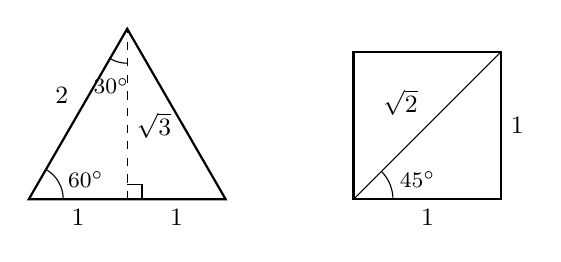
\begin{tikzpicture}[scale=1.25, every node/.style={font=\small}]
  \draw[thick] (0,0) -- (2,0) -- (1,1.732) -- cycle;
  \draw[dashed] (1,0) -- (1,1.732);
  \draw (1,0.15) -- (1.15,0.15) -- (1.15,0);
  \node[below] at (0.5,0) {$1$}; \node[below] at (1.5,0) {$1$};
  \node[above left] at (0.5,0.87) {$2$};
  \node[right] at (1,0.75) {$\sqrt{3}$};
  \draw (0.35,0) arc (0:60:0.35); \node at (0.58,0.2) {\footnotesize$60^\circ$};
  \draw (1,1.382) arc (270:240:0.35); \node at (0.84,1.15) {\footnotesize$30^\circ$};
  \begin{scope}[xshift=3.3cm]
    \draw[thick] (0,0) rectangle (1.5,1.5);
    \draw (0,0) -- (1.5,1.5);
    \node[below] at (0.75,0) {$1$}; \node[right] at (1.5,0.75) {$1$};
    \node[above left] at (0.75,0.75) {$\sqrt{2}$};
    \draw (0.4,0) arc (0:45:0.4); \node at (0.65,0.2) {\footnotesize$45^\circ$};
  \end{scope}
\end{tikzpicture}
\end{center}

Leyendo las razones en esas dos figuras se obtiene la tabla de valores exactos:

\begin{center}
{\renewcommand{\arraystretch}{1.6}
\begin{tabular}{cccc}
  \toprule
  $\theta$ & $\sen\theta$ & $\cos\theta$ & $\tg\theta$\\
  \midrule
  $30^\circ$ & $\frac{1}{2}$ & $\frac{\sqrt{3}}{2}$ & $\frac{\sqrt{3}}{3}$\\
  $45^\circ$ & $\frac{\sqrt{2}}{2}$ & $\frac{\sqrt{2}}{2}$ & $1$\\
  $60^\circ$ & $\frac{\sqrt{3}}{2}$ & $\frac{1}{2}$ & $\sqrt{3}$\\
  \bottomrule
\end{tabular}}
\end{center}

Observa que $\sen 30^\circ = \cos 60^\circ$ y $\sen 60^\circ = \cos 30^\circ$: el
cateto opuesto a un ángulo es el adyacente al otro, porque $30^\circ$ y
$60^\circ$ son complementarios. $\sqrt{2}$ y $\sqrt{3}$ son irracionales: los
valores exactos se dejan con la raíz.

\begin{aplicacion}[Las escuadras de dibujo]
Las dos escuadras del juego de geometría son justamente estos triángulos: la
de $45^\circ$ y la de $30^\circ$--$60^\circ$. Con ellas, arquitectos y
dibujantes técnicos trazan sin transportador las inclinaciones más usadas en
planos y en dibujos en perspectiva.
\end{aplicacion}

\begin{preguntas}
% Ejercicio: razones-trigonometricas-10-054
\pregunta Un hexágono regular está inscrito en un círculo de radio $4$. Encuentra su
perímetro $P$ y su área $A$. (Pista: se divide en seis triángulos equiláteros;
¿por qué la cuerda de $60^\circ$ mide lo mismo que el radio?)
\espacio{3cm}
% Ejercicio: razones-trigonometricas-10-056
\pregunta Encuentra el área de una estrella de David regular (estrella de $6$ puntas
formada por dos triángulos equiláteros) inscrita en un círculo de radio $1$.
\espacio{3.5cm}
\end{preguntas}

\begin{resumen}
\begin{itemize}
  \item $30^\circ$ y $60^\circ$ salen del triángulo equilátero partido (lados $1$, $\sqrt{3}$, $2$);
        $45^\circ$, del cuadrado partido (lados $1$, $1$, $\sqrt{2}$).
  \item Si $\alpha + \beta = 90^\circ$, entonces $\sen\alpha = \cos\beta$.
  \item Las razones no se suman como los ángulos: $\sen(30^\circ + 30^\circ) \neq 2\sen 30^\circ$.
\end{itemize}
\end{resumen}

% ---------------------------------------------------------------------
\tema{Resolución de triángulos rectángulos}\label{tema:resolucion}

\begin{hilo}
Alejandría, hacia el año 400. Hipatia revisa el comentario de su padre al
\emph{Almagesto}, lleno de cálculos con cuerdas. Un error en una cifra se
propaga a todas las que siguen. Resolver un triángulo es también eso: hallar
cada parte con cuidado y comprobarla.
\end{hilo}

\textbf{Resolver} un triángulo es hallar todos sus lados y ángulos. En un
triángulo rectángulo ($\gamma = 90^\circ$, hipotenusa $c$, catetos $a$ y $b$
opuestos a $\alpha$ y $\beta$) basta conocer \textbf{dos datos, uno de ellos un
lado}:
\begin{itemize}
  \item los ángulos agudos suman $90^\circ$: $\beta = 90^\circ - \alpha$;
  \item con un ángulo y un lado se usa la razón que relaciona el lado conocido con el buscado;
  \item con dos lados, se halla un ángulo con la razón inversa y el tercer lado con Pitágoras.
\end{itemize}

% Ejercicio: razones-trigonometricas-10-020
\begin{ejemplo}[Un ángulo y la hipotenusa]
Resolver el triángulo con $\alpha = \num{56,2}^\circ$ y $c = \num{91,3}$:
$\beta = 90^\circ - \num{56,2}^\circ = \num{33,8}^\circ$;
$a = \num{91,3}\sen \num{56,2}^\circ \approx \num{75,9}$;
$b = \num{91,3}\cos \num{56,2}^\circ \approx \num{50,8}$.
Las respuestas se dan con tres cifras significativas, como los datos.
\end{ejemplo}

% Ejercicio: razones-trigonometricas-10-028
\begin{ejemplo}[Dos catetos]
Resolver el triángulo con $a = \num{9,52}$ y $b = \num{14,7}$:
$\tg\alpha = \frac{\num{9,52}}{\num{14,7}}$, así que $\alpha \approx \num{32,9}^\circ$
y $\beta \approx \num{57,1}^\circ$; $c = \sqrt{\num{9,52}^2 + \num{14,7}^2} \approx \num{17,51}$.
\end{ejemplo}

\begin{aplicacion}[Cifras significativas]
En ingeniería y topografía, un resultado no puede ser más preciso que los datos
con que se calculó. Si un ángulo se midió a la décima de grado, dar un lado con
seis decimales es inventar precisión: se redondea al número de cifras de los
datos.
\end{aplicacion}

\begin{preguntas}
% Ejercicio: razones-trigonometricas-10-019, razones-trigonometricas-10-022
\Needspace{8\baselineskip}
\pregunta Resuelve el triángulo rectángulo ($\gamma = 90^\circ$). Dibújalo primero y
marca sus partes.
\begin{opciones*}(2)
  \item $\alpha = 42^\circ$, $c = 35$
  \item $\beta = 29^\circ$, $c = 50$
\end{opciones*}
\espacio{3.5cm}
% Ejercicio: razones-trigonometricas-10-025, razones-trigonometricas-10-030
\pregunta Resuelve el triángulo rectángulo ($\gamma = 90^\circ$, hipotenusa $c$):
\begin{opciones*}(2)
  \item $a = 9$, $b = 12$
  \item $c = 41$, $a = 40$
\end{opciones*}
\espacio{3.5cm}
% Ejercicio: razones-trigonometricas-10-021, razones-trigonometricas-10-046
\pregunta Resuelve el triángulo rectángulo ($\gamma = 90^\circ$, hipotenusa $c$):
\begin{opciones*}(2)
  \item $\alpha = \num{39,4}^\circ$, $a = 120$
  \item $b = \num{67,3}$, $c = \num{82,9}$
\end{opciones*}
\espacio{3.5cm}
\end{preguntas}

\begin{resumen}
\begin{itemize}
  \item Con dos datos (al menos un lado) se resuelve cualquier triángulo rectángulo.
  \item Elige la razón que tiene el dato conocido y la incógnita; usa Pitágoras para comprobar.
  \item Redondea según la precisión de los datos.
\end{itemize}
\end{resumen}

% ---------------------------------------------------------------------
\tema{Aplicaciones del triángulo rectángulo}\label{tema:aplicaciones}

\begin{hilo}
Llanura de Yaruquí, cerca de Quito, 1736. Jorge Juan, Antonio de Ulloa y los
académicos franceses miden con cadenas una base de más de 12~km. Es la única
distancia que medirán directamente: desde sus extremos apuntan a señales en
las montañas y, con ángulos, calculan las demás.
\end{hilo}

El \textbf{ángulo de elevación} es el que forma la visual con la horizontal
cuando se mira hacia arriba; el \textbf{ángulo de depresión}, cuando se mira
hacia abajo. Casi todos los problemas de medición indirecta se reducen a uno o
dos triángulos rectángulos con una distancia conocida.

% Ejercicio: razones-trigonometricas-10-018
\begin{ejemplo}[Un poste visto desde dos puntos]
Desde el pie $P$ de un poste vertical se mide sobre el suelo horizontal: a $15$
unidades de $P$ el ángulo de elevación a la punta es $44^\circ$, y a $15 + x$
unidades (en la misma dirección) es $24^\circ$. La altura es
$h = 15\tg 44^\circ \approx \num{14,49}$; en el triángulo grande,
$15 + x = \frac{h}{\tg 24^\circ}$, así que $x = \frac{15\tg 44^\circ}{\tg 24^\circ} - 15 \approx \num{17,5}$.

\begin{center}
\begin{tikzpicture}[scale=0.3, every node/.style={font=\small}]
  \draw[thick] (-32.5,0) -- (0,0);
  \draw[very thick] (0,0) -- (0,14.49);
  \draw (-15,0) -- (0,14.49);
  \draw (-32.5,0) -- (0,14.49);
  \draw (-0.8,0) -- (-0.8,0.8) -- (0,0.8);
  \node[right] at (0,7.2) {$h$};
  \node[below right] at (0,0) {$P$};
  \node[below] at (-7.5,0) {$15$};
  \node[below] at (-23.75,0) {$x$};
  \fill (-15,0) circle (4pt); \fill (-32.5,0) circle (4pt);
  \draw (-11,0) arc (0:44:4); \node at (-9.5,1.4) {\footnotesize$44^\circ$};
  \draw (-26.5,0) arc (0:24:6); \node at (-24.3,1.1) {\footnotesize$24^\circ$};
\end{tikzpicture}
\end{center}
\end{ejemplo}

\begin{aplicacion}[El clinómetro casero]
Un transportador, un pitillo pegado a su borde y una cuerda con un peso colgando
del centro forman un \emph{clinómetro}: se mira la punta de un árbol o de un
edificio por el pitillo y la cuerda marca el ángulo. Midiendo la distancia al
pie con un metro y sumando la altura de los ojos, se calcula la altura sin
subirse. Los topógrafos hacen lo mismo con un teodolito.
\end{aplicacion}

\begin{preguntas}
% Ejercicio: razones-trigonometricas-10-033
\pregunta Una trayectoria recta que sube una colina se eleva $26$ pies por cada
$100$ pies horizontales. ¿Qué ángulo forma con la horizontal? ¿Cambia la
respuesta si las medidas estuvieran en metros?
\espacio{2.5cm}
% Ejercicio: razones-trigonometricas-10-050
\pregunta Desde la ventana de un edificio de oficinas se ve una torre de televisión
a $600$~m de distancia horizontal. El ángulo de elevación de la punta de la torre
es $\num{19,6}^\circ$ y el ángulo de depresión de su base es $\num{21,3}^\circ$. ¿Qué
altura tiene la torre?
\espacio{3cm}
% Ejercicio: razones-trigonometricas-10-017
\Needspace{10\baselineskip}
\pregunta Dos triángulos rectángulos comparten un cateto vertical de longitud $20$.
En uno, ese cateto es opuesto a un ángulo de $26^\circ$; en el otro, es opuesto a
un ángulo de $38^\circ$. Los catetos horizontales están sobre la misma recta, uno a
cada lado del cateto común, y juntos miden $x$. Halla $x$. (Así avanzaba la
cadena de triángulos de la Misión Geodésica: cada lado calculado era la base
del triángulo siguiente.)
\espacio{3cm}
% Ejercicio: razones-trigonometricas-10-053
\pregunta Encuentra el ángulo entre una diagonal principal de un cubo y la diagonal
de una de sus caras que parte del mismo vértice.
\espacio{3cm}
\end{preguntas}

\begin{resumen}
\begin{itemize}
  \item Dibuja el esquema, marca la distancia conocida y los ángulos, y busca los triángulos rectángulos.
  \item Elevación: se mira hacia arriba desde la horizontal; depresión: hacia abajo.
  \item Con dos ángulos, se plantean dos triángulos y se combinan (sumando, restando o sustituyendo).
\end{itemize}
\end{resumen}

% ---------------------------------------------------------------------
\tema{Ángulos como rotación}\label{tema:rotacion}

\begin{hilo}
Desde Rodas, Hiparco mira un cielo que gira: las estrellas dan una vuelta
completa cada día alrededor del polo. Para medir esos giros usa un círculo
dividido en $360$ grados, la misma división de su tabla de cuerdas. Un ángulo
ya no es solo una esquina: es cuánto ha girado algo.
\end{hilo}

En trigonometría, un ángulo es la \textbf{rotación} de un rayo alrededor de su
extremo, desde un \emph{lado inicial} hasta un \emph{lado terminal}. Si gira en
sentido contrario a las manecillas del reloj, el ángulo es \textbf{positivo}; si
gira en el sentido de las manecillas, es \textbf{negativo}. Un ángulo está en
\textbf{posición estándar} si su vértice está en el origen y su lado inicial es
el semieje $x$ positivo. Los ángulos que tienen el mismo lado terminal se
llaman \textbf{coterminales}: se diferencian en un número entero de vueltas,
$\theta + 360^\circ k$.

\begin{center}
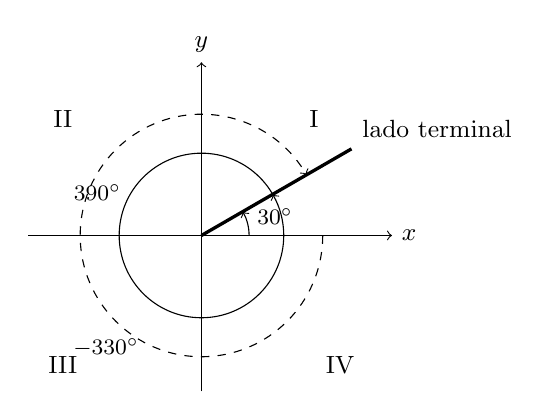
\begin{tikzpicture}[scale=1.1, every node/.style={font=\small}]
  \draw[->] (-2,0) -- (2.2,0) node[right] {$x$};
  \draw[->] (0,-1.8) -- (0,2) node[above] {$y$};
  \draw[very thick] (0,0) -- (30:2) node[above right] {lado terminal};
  \draw[->] (0.55,0) arc (0:30:0.55); \node at (0.85,0.22) {\footnotesize$30^\circ$};
  \draw[->] (0.95,0) arc (0:390:0.95); \node at (-1.2,0.5) {\footnotesize$390^\circ$};
  \draw[->, dashed] (1.4,0) arc (0:-330:1.4); \node at (-1.1,-1.3) {\footnotesize$-330^\circ$};
  \node at (1.3,1.35) {I}; \node at (-1.6,1.35) {II}; \node at (-1.6,-1.5) {III}; \node at (1.6,-1.5) {IV};
\end{tikzpicture}

{\small $30^\circ$, $390^\circ$ y $-330^\circ$ tienen el mismo lado terminal: son coterminales.}
\end{center}

\textbf{Grados, minutos y segundos.} Desde los babilonios, cada grado se divide
en $60$ minutos ($60'$) y cada minuto en $60$ segundos ($60''$). Así,
$40^\circ\,30' = \num{40,5}^\circ$, y el ángulo de Eratóstenes,
$7^\circ\,12'$, es $\num{7,2}^\circ$. La calculadora trabaja con grados decimales.

\begin{aplicacion}[La Tierra gira $15^\circ$ por hora]
La Tierra da una vuelta sobre su eje en unas 24 horas: $\frac{360^\circ}{24} =
15^\circ$ por hora. Por eso los husos horarios se separan unos $15^\circ$ de
longitud, y Colombia (hacia los $75^\circ$ oeste) tiene cinco horas menos que
Greenwich.
\end{aplicacion}

\begin{preguntas}
% Ejercicio: circulo-unitario-10-028, circulo-unitario-10-032
\pregunta Resta (o suma) vueltas completas para hallar un ángulo coterminal entre
$0^\circ$ y $360^\circ$, ubícalo en los ejes y halla el valor exacto sin calculadora:
\begin{opciones*}(2)
  \item $\cos(-720^\circ)$
  \item $\sen(900^\circ)$
\end{opciones*}
\espacio{2.5cm}
% Ejercicio: angulos-radianes-10-035
\pregunta ¿Cuántos radianes recorre el minutero de un reloj en $1$ hora? ¿Y el horario
en $1$ hora? ¿Y el minutero en $5$ horas? (Recuerda que una vuelta son $2\pi$
radianes.) ¿Qué signo tienen esos giros según la convención de esta sección?
\espacio{2.5cm}
\end{preguntas}

\begin{resumen}
\begin{itemize}
  \item Un ángulo es un giro: positivo en sentido antihorario, negativo en sentido horario.
  \item Posición estándar: vértice en el origen, lado inicial en el semieje $x$ positivo.
  \item Coterminales: $\theta + 360^\circ k$. Para ubicar un ángulo grande, se le restan vueltas.
\end{itemize}
\end{resumen}

% ---------------------------------------------------------------------
\tema{Radianes}\label{tema:radianes}

\begin{hilo}
Eratóstenes no dijo «siete grados»: dijo que el ángulo de la sombra era
$\frac{1}{50}$ de la vuelta completa. Medir un ángulo como una parte de la
vuelta, o mejor, comparando el arco con el radio, es la idea del radián.
\end{hilo}

\begin{definicion}[Radián]
Un ángulo central mide \textbf{un radián} si el arco que recorta en la
circunferencia mide lo mismo que el radio. Como la circunferencia mide $2\pi r$,
en una vuelta caben $2\pi$ radianes:
\[
  360^\circ = 2\pi \text{ rad}, \qquad 180^\circ = \pi \text{ rad}, \qquad
  1 \text{ rad} = \frac{180^\circ}{\pi} \approx \num{57,3}^\circ.
\]
\end{definicion}

\begin{center}
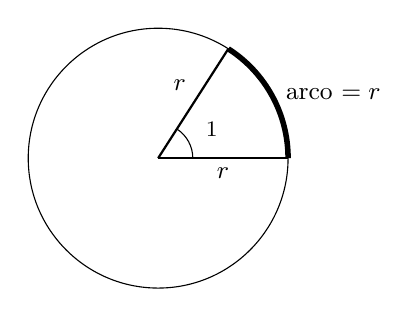
\begin{tikzpicture}[scale=1.1, every node/.style={font=\small}]
  \draw (0,0) circle (1.5);
  \draw[thick] (0,0) -- (1.5,0);
  \draw[thick] (0,0) -- (57.3:1.5);
  \draw[line width=2pt] (1.5,0) arc (0:57.3:1.5);
  \node[below] at (0.75,0) {$r$};
  \node[above left] at (57.3:0.8) {$r$};
  \node[right] at (28.6:1.55) {arco $= r$};
  \draw (0.4,0) arc (0:57.3:0.4); \node at (28:0.7) {\footnotesize$1$};
\end{tikzpicture}
\end{center}

Para convertir: de grados a radianes se multiplica por $\frac{\pi}{180}$; de
radianes a grados, por $\frac{180^\circ}{\pi}$. Los ángulos especiales:
$30^\circ = \frac{\pi}{6}$, $45^\circ = \frac{\pi}{4}$, $60^\circ = \frac{\pi}{3}$,
$90^\circ = \frac{\pi}{2}$.

% Ejercicio: angulos-radianes-10-070
\begin{ejemplo}[Conversiones]
$33^\circ = 33\cdot\frac{\pi}{180} = \frac{11\pi}{60} \approx \num{0,576}$ rad, y
$\frac{9\pi}{4}$ rad $= \frac{9\pi}{4}\cdot\frac{180^\circ}{\pi} = 405^\circ$.
\end{ejemplo}

\begin{aplicacion}[La calculadora en modo RAD]
Las calculadoras, las hojas de cálculo y los lenguajes de programación usan
radianes por defecto: en una hoja de cálculo, \texttt{=SENO(30)} no da $0{,}5$,
porque interpreta $30$ radianes. Hay que escribir \texttt{=SENO(RADIANES(30))}.
\end{aplicacion}

\begin{preguntas}
% Ejercicio: angulos-radianes-10-001, angulos-radianes-10-003, angulos-radianes-10-010
\pregunta Convierte a radianes (puedes dejar $\pi$ en la respuesta):
\begin{opciones*}(3)
  \item $120^\circ$
  \item $315^\circ$
  \item $-420^\circ$
\end{opciones*}
\espacio{2cm}
% Ejercicio: angulos-radianes-10-017, angulos-radianes-10-022
\pregunta Convierte a grados (a la décima de grado):
\begin{opciones*}(2)
  \item $\dfrac{14}{3}\pi$ radianes
  \item $3$ radianes
\end{opciones*}
\espacio{2cm}
% Ejercicio: angulos-radianes-10-049, angulos-radianes-10-050
\pregunta Convierte a radianes:
\begin{opciones*}(2)
  \item $23$ revoluciones
  \item $\left(\dfrac{60}{\pi}\right)^\circ$
\end{opciones*}
\espacio{2cm}
\end{preguntas}

\begin{resumen}
\begin{itemize}
  \item Un radián es el ángulo central cuyo arco mide un radio: $1$ rad $\approx \num{57,3}^\circ$.
  \item $180^\circ = \pi$ rad. Grados $\to$ radianes: $\times\frac{\pi}{180}$; radianes $\to$ grados: $\times\frac{180^\circ}{\pi}$.
  \item Antes de usar la calculadora, revisa si está en DEG o en RAD.
\end{itemize}
\end{resumen}

% ---------------------------------------------------------------------
\tema{Arco y sector circular}\label{tema:arcosector}

\begin{hilo}
Si el ángulo entre Siena y Alejandría es $\frac{1}{50}$ de la vuelta, el arco
entre las dos ciudades es $\frac{1}{50}$ de la circunferencia de la Tierra.
Eratóstenes solo necesitó multiplicar. Dos mil años después, la Misión Geodésica
midió un arco de unos tres grados en los Andes para saber cuánto mide un grado
cerca del ecuador.
\end{hilo}

Si un ángulo central de $t$ radianes corta un círculo de radio $r$, el
\textbf{arco} y el \textbf{sector} que determina miden
\[
  s = r\,t, \qquad A = \tfrac{1}{2}\,r^2\,t \qquad (t \text{ en radianes}).
\]
La fórmula del arco sale de la definición: cada radián recorta un arco de
longitud $r$. La del sector, de una proporción: el sector es la fracción
$\frac{t}{2\pi}$ del círculo, así que $A = \frac{t}{2\pi}\cdot\pi r^2$.

\begin{center}
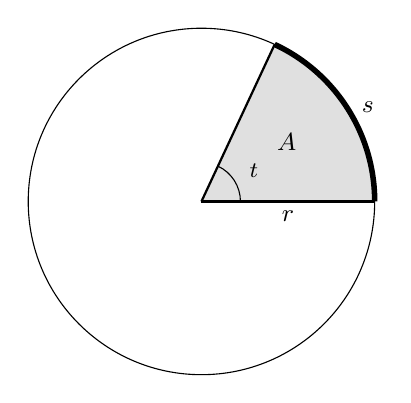
\begin{tikzpicture}[scale=1.1, every node/.style={font=\small}]
  \fill[black!12] (0,0) -- (0:2) arc (0:65:2) -- cycle;
  \draw (0,0) circle (2);
  \draw[thick] (0,0) -- (2,0); \draw[thick] (0,0) -- (65:2);
  \draw[line width=2pt] (2,0) arc (0:65:2);
  \node[below] at (1,0) {$r$};
  \node[right] at (32:2.05) {$s$};
  \node at (35:1.2) {$A$};
  \draw (0.45,0) arc (0:65:0.45); \node at (30:0.7) {\footnotesize$t$};
\end{tikzpicture}
\end{center}

% Ejercicio: angulos-radianes-10-071
\begin{ejemplo}[Una rueda que avanza]
Cada vuelta de una rueda de $30$~cm de radio es un ángulo de $2\pi$ y avanza un
arco $s = 30 \cdot 2\pi$~cm. En $100$ vueltas avanza
$d = 100 \cdot 2\pi \cdot 30 = 6000\pi \approx 18\,850$~cm $\approx \num{188,5}$~m.
\end{ejemplo}

\begin{aplicacion}[Un grado de meridiano]
Si la Tierra es una esfera de unos $6371$~km de radio, el arco de meridiano de
$1^\circ$ mide $s = 6371 \cdot \frac{\pi}{180} \approx 111$~km. Por eso en los mapas
un grado de latitud equivale a unos $111$~km, y la milla náutica de los barcos y
aviones es el arco de un minuto de latitud.
\end{aplicacion}

\begin{preguntas}
% Ejercicio: angulos-radianes-10-033
\pregunta Encuentra el radio $r$ de un círculo en el que un ángulo central de
$t = \num{2,8}$ radianes abarca un arco de $s = \num{8,4}$~cm.
\espacio{2cm}
% Ejercicio: angulos-radianes-10-054, angulos-radianes-10-056
\pregunta Encuentra la longitud del arco que abarca, en un círculo de radio
$\num{4,25}$~cm, un ángulo central de:
\begin{opciones*}(2)
  \item $6$ radianes
  \item $\dfrac{17\pi}{6}$ radianes
\end{opciones*}
\espacio{2cm}
% Ejercicio: angulos-radianes-10-058
\pregunta El piñón del pedal de la bicicleta de María tiene $12$~cm de radio, el de
la rueda trasera $3$~cm y las ruedas $40$~cm de radio. ¿Qué distancia recorre María
si da $30$ vueltas completas al pedal?
\espacio{3cm}
% Ejercicio: angulos-radianes-10-068
\pregunta Un cono tiene base de radio $R$ y generatriz (altura inclinada) $L$.
Encuentra la fórmula de su superficie lateral. Sugerencia: imagina que el cono es
de papel, córtalo a lo largo de una generatriz y extiéndelo sobre una mesa.
\espacio{3.5cm}
\end{preguntas}

\begin{resumen}
\begin{itemize}
  \item Arco: $s = rt$; sector: $A = \frac{1}{2}r^2 t$, con $t$ \textbf{en radianes}.
  \item Si el ángulo está en grados, primero se convierte a radianes.
  \item Un ángulo es la fracción $\frac{t}{2\pi}$ de la vuelta: el arco y el área son esa misma fracción del total.
\end{itemize}
\end{resumen}

% ---------------------------------------------------------------------
\tema{Círculo unitario}\label{tema:circulounitario}

\begin{hilo}
Nueva Granada, 1850. Agustín Codazzi empieza a recorrer el país para levantar
sus mapas. Cada lugar queda descrito por dos ángulos: su latitud y su
longitud. Localizar un punto con un ángulo es lo que hace el círculo unitario.
\end{hilo}

El \textbf{círculo unitario} es el círculo de radio $1$ con centro en el origen.
En él, un ángulo $t$ en radianes recorta un arco de longitud $s = 1\cdot t = t$:
\emph{la medida en radianes es la longitud del arco}. A cada ángulo $\theta$ en
posición estándar le corresponde el punto $P$ donde su lado terminal corta el
círculo.

Si $\theta$ es agudo, al bajar una perpendicular desde $P$ se forma un triángulo
rectángulo de hipotenusa $1$, así que sus catetos miden $\cos\theta$ y
$\sen\theta$:
\[
  P(\theta) = (\cos\theta,\ \sen\theta).
\]
Esta igualdad sirve de definición para cualquier ángulo, también los no agudos:
es lo que estudiaremos en el trimestre II. Por ahora basta con los ángulos
agudos y con los que caen sobre los ejes: $P(0) = (1, 0)$,
$P\left(\frac{\pi}{2}\right) = (0, 1)$, $P(\pi) = (-1, 0)$ y
$P\left(\frac{3\pi}{2}\right) = (0, -1)$; los ángulos coterminales tienen el mismo punto.

\begin{center}
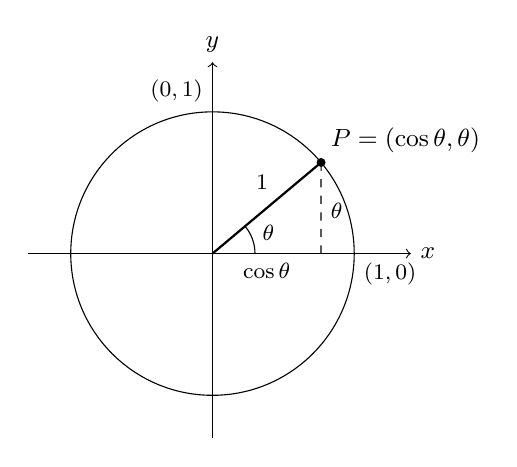
\begin{tikzpicture}[scale=1.8, every node/.style={font=\small}]
  \draw[->] (-1.3,0) -- (1.4,0) node[right] {$x$};
  \draw[->] (0,-1.3) -- (0,1.35) node[above] {$y$};
  \draw (0,0) circle (1);
  \draw[thick] (0,0) -- (40:1);
  \draw[dashed] (40:1) -- (0.766,0);
  \fill (40:1) circle (0.9pt) node[above right] {$P = (\cos\theta, \sen\theta)$};
  \draw (0.3,0) arc (0:40:0.3); \node at (20:0.42) {\footnotesize$\theta$};
  \node[below] at (0.383,0) {\footnotesize$\cos\theta$};
  \node[right] at (0.766,0.3) {\footnotesize$\sen\theta$};
  \node[above left] at (40:0.6) {\footnotesize$1$};
  \node[below right] at (1,0) {\footnotesize$(1,0)$};
  \node[above left] at (0,1) {\footnotesize$(0,1)$};
\end{tikzpicture}
\end{center}

\begin{aplicacion}[Latitud y longitud]
En un mapa, Cali está hacia los $3^\circ\,27'$ norte y los $76^\circ\,32'$ oeste.
Ambas coordenadas son ángulos medidos desde el centro de la Tierra: la latitud,
desde el ecuador; la longitud, desde el meridiano de Greenwich. Los receptores
GPS entregan la posición justamente así.
\end{aplicacion}

\begin{preguntas}
% Ejercicio: circulo-unitario-10-017, circulo-unitario-10-018, circulo-unitario-10-019, circulo-unitario-10-020
\pregunta Usa el círculo unitario (sin calculadora) para hallar el valor exacto:
\begin{opciones*}(4)
  \item $\sen\left(\frac{5\pi}{2}\right)$
  \item $\cos(7\pi)$
  \item $\sen(-4\pi)$
  \item $\cos\left(\frac{7\pi}{2}\right)$
\end{opciones*}
\espacio{2cm}
% Ejercicio: angulos-radianes-10-036, angulos-radianes-10-037, angulos-radianes-10-038
\Needspace{8\baselineskip}
\pregunta Un punto $P$ se mueve sobre el círculo unitario en sentido contrario a
las manecillas del reloj, empezando en $(1, 0)$. ¿En qué cuadrante está $P$ cuando
ha recorrido estas distancias?
\begin{opciones*}(3)
  \item $3$ unidades
  \item $\num{4,8}$ unidades
  \item $100$ unidades
\end{opciones*}
\espacio{2.5cm}
\end{preguntas}

\begin{resumen}
\begin{itemize}
  \item En el círculo unitario, la medida en radianes es la longitud del arco.
  \item El punto del ángulo $\theta$ es $P(\theta) = (\cos\theta, \sen\theta)$, y cumple $\cos^2\theta + \sen^2\theta = 1$.
  \item $P(0) = (1, 0)$, $P(\frac{\pi}{2}) = (0, 1)$, $P(\pi) = (-1, 0)$, $P(\frac{3\pi}{2}) = (0, -1)$.
\end{itemize}
\end{resumen}

% ---------------------------------------------------------------------
% 5. Saber 11
% ---------------------------------------------------------------------
\seccion{Prepárate para Saber 11}

\begin{instrucciones}
Preguntas de selección múltiple con única respuesta, como las de la prueba
Saber 11. Son las preguntas 44, 22 y 23 del cuadernillo de preguntas liberado
por el Icfes en 2026, reproducidas textualmente con sus figuras~\cite{icfes2026}.
\end{instrucciones}

\begin{preguntas}
% Ejercicio: icfes-cuadernillo-2026-044
\pregunta En un parque hay una rueda giratoria de 3 m de radio. La rueda está
diseñada para 10 personas, cada una en un sector circular de igual área, como
muestra la figura.
\begin{center}
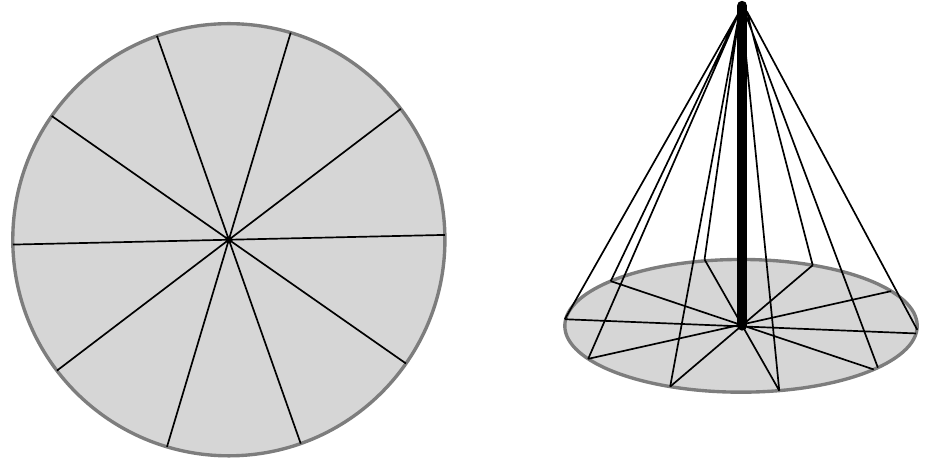
\includegraphics[width=0.3\linewidth]{figuras/icfes-2026-pregunta-44.png}
\end{center}
Para determinar el área que le corresponde a cada persona, se divide $2\pi$
entre 10 lo que determina el ángulo $\theta$ de cada sector y se usa la fórmula
del área de un sector circular $S$: $S = r^2\,\frac{\theta}{2}$ donde $r$ es el
radio de la circunferencia. Utilizando una aproximación de $\pi = 3$, ¿cuál es
el área aproximada que le corresponde a cada persona?
\begin{opciones*}(4)
  \item $\num{3,6}$ m²
  \item $\num{2,7}$ m²
  \item $\num{9,0}$ m²
  \item $\num{1,8}$ m²
\end{opciones*}
% Ejercicio: icfes-cuadernillo-2026-022
\Needspace{24\baselineskip}
\pregunta La línea punteada en la figura muestra un corte realizado a un
triángulo. El corte es paralelo a la base y corta por la mitad a la altura, $h$,
que es perpendicular a la base.
\begin{center}
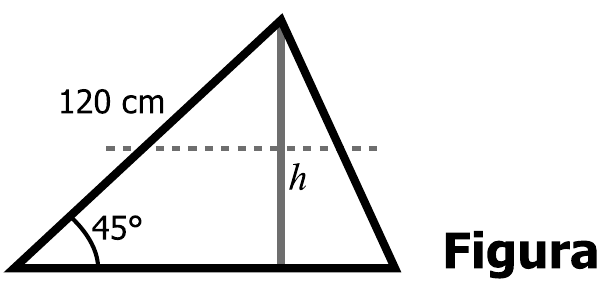
\includegraphics[width=0.4\linewidth]{figuras/icfes-2026-pregunta-22.png}
\end{center}
Para realizar el corte, se determinó la altura del triángulo usando la fórmula
$\sen(45^\circ) = \frac{h}{120}$; luego se dividió h entre dos. Realizando este
procedimiento, y teniendo en cuenta que
$\sen(45^\circ) = \frac{\sqrt{2}}{2} \approx \num{0,71}$, ¿cuál fue, aproximadamente,
la distancia a la que se cortó la altura del triángulo?
\begin{opciones*}(4)
  \item 85 cm.
  \item 60 cm.
  \item 42 cm.
  \item 30 cm.
\end{opciones*}
% Ejercicio: icfes-cuadernillo-2026-023
\pregunta Un cartabón es una plantilla que se utiliza en dibujo técnico y que
tiene forma de triángulo rectángulo escaleno, de modo que su hipotenusa mide el
doble del cateto de menor longitud.
\begin{center}
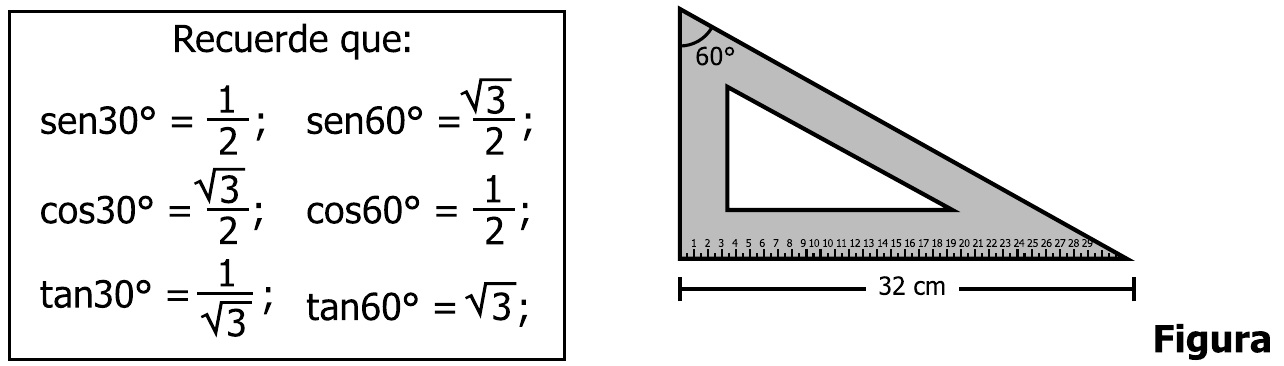
\includegraphics[width=0.65\linewidth]{figuras/icfes-2026-pregunta-23.png}
\end{center}
Si el cateto más largo de un cartabón mide 32 centímetros, como muestra la
figura, ¿cuál de las siguientes medidas corresponde a su cateto menor?
\begin{opciones*}(4)
  \item 16 cm.
  \item $\dfrac{32}{\sqrt{3}}$ cm.
  \item 27 cm.
  \item $\dfrac{64}{\sqrt{3}}$ cm.
\end{opciones*}
\end{preguntas}

% ---------------------------------------------------------------------
% 6. Cierre del hilo conductor
% ---------------------------------------------------------------------
\seccion{Cierre: de una sombra a un mapa}

Tales comparó dos sombras; Eratóstenes, dos ángulos en dos ciudades; Hiparco
puso en una tabla las cuerdas de un círculo, y Hipatia revisó los cálculos que
las usaban. Con esas ideas, Jorge Juan, Ulloa y los académicos franceses
midieron la forma de la Tierra desde los Andes, y Codazzi levantó los mapas de
nuestro país. La lección es siempre la misma: con un lado conocido y unos
ángulos, lo inalcanzable se puede medir. En el segundo trimestre recorreremos
el círculo unitario completo: ángulos mayores de $90^\circ$, signos en cada
cuadrante y las otras funciones trigonométricas.

% ---------------------------------------------------------------------
% 7. Evaluación (secciones institucionales)
% ---------------------------------------------------------------------
\matrizevaluacion
  {Define seno, coseno y tangente y explica por qué dependen solo del ángulo;
   conoce los valores exactos de $30^\circ$, $45^\circ$ y $60^\circ$ y relaciona grados,
   radianes y arcos.}
  {Resuelve triángulos rectángulos y problemas de medición indirecta; convierte
   ángulos, calcula arcos y sectores y ubica puntos en el círculo unitario.}
  {Revisa sus cálculos y los de sus compañeros: unidades, modo de la calculadora
   y redondeo.}
  {Trabaja en equipo en la medición del patio y valora el trabajo colectivo de
   las expediciones científicas, incluida la de mujeres como Hipatia.}

\autoevaluacion

\seguimientodocente

% ---------------------------------------------------------------------
% 8. Referencias
% ---------------------------------------------------------------------
\begin{referencias}
% verificado: https://www.bibliotecanacional.gov.co/es-co/colecciones/biblioteca-digital/mapeando/Paginas/capitulocinco.html — contrato del 1 ene. 1850; Codazzi nació en Lugo en 1793 y murió el 7 feb. 1859; Carta y Atlas de 1865
\bibitem{bnc} Biblioteca Nacional de Colombia (s.\,f.). La Comisión Corográfica: un
  vasto esfuerzo para la construcción de una nación. En \emph{Mapeando}, cap.~5. Bogotá.
% verificado: https://grbs.library.duke.edu/article/view/4171 — Greek, Roman and Byzantine Studies 31 (1990), pp. 103–127
\bibitem{cameron1990} Cameron, A. (1990). Isidore of Miletus and Hypatia: On the
  editing of mathematical texts. \emph{Greek, Roman and Byzantine Studies}, 31, 103--127.
% verificado: https://it.wikisource.org/wiki/Il_Saggiatore/6 — Il Saggiatore (Roma: Giacomo Mascardi, 1623), cap. 6; ficha de la edición en https://portalegalileo.museogalileo.it/egjr.asp?c=36261
\bibitem{galileo1623} Galilei, G. (1623). \emph{Il Saggiatore}. Roma: Giacomo Mascardi.
% verificado: recursos/matematicas/icfes/09-Marzo_Cuadernillo-de-Preguntas-Matematicas-Saber-11-2026.pdf (archivo local) — preguntas 22 y 23 (p. 17) y 44 (p. 29); claves C, B y B
\bibitem{icfes2026} Icfes (2026). \emph{Cuadernillo de preguntas Saber 11.º: Prueba
  de Matemáticas} (marzo de 2026), preguntas 22, 23 y 44. Bogotá: Icfes.
% verificado: https://mathshistory.st-andrews.ac.uk/Biographies/Eratosthenes/ — 276–194 a. C.; Siena y Alejandría; 7°12′; 250 000 estadios; Cleómedes, Teón de Esmirna, Estrabón; estadio de 157,2 a 166,7 m
\bibitem{mactutoreratostenes} MacTutor History of Mathematics (s.\,f.).
  \emph{Eratosthenes of Cyrene}. University of St Andrews.
% verificado: https://mathshistory.st-andrews.ac.uk/Biographies/Hipparchus/ — c. 190–120 a. C., Rodas; tabla de cuerdas; «some historians go so far as to say that trigonometry was invented by him»
\bibitem{mactutorhiparco} MacTutor History of Mathematics (s.\,f.).
  \emph{Hipparchus of Rhodes}. University of St Andrews.
% verificado: https://mathshistory.st-andrews.ac.uk/Biographies/Hypatia/ — ayudó a Teón con su comentario en once libros al Almagesto; murió en Alejandría en 415
\bibitem{mactutorhipatia} MacTutor History of Mathematics (s.\,f.).
  \emph{Hypatia of Alexandria}. University of St Andrews.
% verificado: https://mathshistory.st-andrews.ac.uk/Biographies/Santacilia/ — Juan y Ulloa en la expedición (1735–1744); base en Yaruquí de más de 12 km; unos 3° de latitud; apoyo a Newton
\bibitem{mactutorjuan} MacTutor History of Mathematics (s.\,f.).
  \emph{Jorge Juan y Santacilia}. University of St Andrews.
% verificado: https://mathshistory.st-andrews.ac.uk/Biographies/La_Condamine/ — sale en abril de 1735 con Bouguer y Godin; Quito el 4 jun. 1736; triangulación Quito–Cuenca; Newton frente a Descartes
\bibitem{mactutorlacondamine} MacTutor History of Mathematics (s.\,f.).
  \emph{Charles-Marie de La Condamine}. University of St Andrews.
% verificado: https://mathshistory.st-andrews.ac.uk/Biographies/Thales/ — altura de las pirámides por la sombra según Jerónimo (en Diógenes Laercio), Plinio y Plutarco
\bibitem{mactutortales} MacTutor History of Mathematics (s.\,f.).
  \emph{Thales of Miletus}. University of St Andrews.
% verificado: https://gblumen.mineducacion.gov.co/cgi-bin/koha/opac-detail.pl?biblionumber=4785 — MEN 2016
\bibitem{mendba} Ministerio de Educación Nacional (2016). \emph{Derechos Básicos de
  Aprendizaje V.2: Matemáticas}. Bogotá: MEN.
% verificado: recursos/matematicas/Guías pedagógicas Matemáticas/10 - Modulo_Matematicas_Decimo.docx (archivo local) — autora y título tomados de la portada
\bibitem{quintero} Quintero Palomino, A. (s.\,f.). \emph{Conceptos de las funciones
  trigonométricas y la resolución de triángulos para el grado 10.º} (Guía de apoyo
  educativo en el área de las matemáticas).
\end{referencias}

\end{document}
